\documentclass[12pt,a4paper]{book}
% ================================
% PRÉAMBULE — Mathématiques 6e
% ================================
%\usepackage[utf8]{inputenc} % <- si vous compilez avec XeLaTeX/LuaLaTeX, commentez cette ligne
\usepackage[T1]{fontenc}
\usepackage[french]{babel}
\usepackage{lmodern}
\usepackage{geometry}
\geometry{top=2.5cm,bottom=2.5cm,left=2.3cm,right=2.3cm}
\usepackage{microtype}
\usepackage{titlesec}
\usepackage{fancyhdr}
\usepackage{enumitem}
\usepackage{amsmath,amssymb,amsfonts,mathtools}
\usepackage{siunitx}
\usepackage{graphicx}
\usepackage{tikz}
\usetikzlibrary{angles,quotes,calc,arrows.meta,shapes.geometric}
\usepackage{pgfplots}
\pgfplotsset{compat=1.18}
\usepackage{hyperref}
\usepackage{xcolor}
\hypersetup{
	colorlinks=true,
	linkcolor=blue!50!black,
	urlcolor=blue!50!black,
	citecolor=blue!50!black
}

% Environnements jolis pour Définition / Exemple / Exercice
\usepackage[most]{tcolorbox}
\tcbset{
    rounded corners,
    boxsep=2ex,
    top=1.5ex,
    bottom=1.5ex,
    left=2.5ex,
    right=7ex,
    before skip=1ex,
    after skip=2ex,
    width=\textwidth,
    boxrule=1pt
}
\newtcolorbox{definitionbox}{
    colback=orange!5!white,
    colframe=orange!70!black,
    title={\textbf{Définition}},
    fonttitle=\bfseries,
    coltitle=black
}
\newtcolorbox{examplebox}{
    colback=green!5!white,
    colframe=green!60!black,
    title={\textbf{Exemple}},
    fonttitle=\bfseries,
    coltitle=black
}
\newtcolorbox{exercisebox}{
    colback=purple!5!white,
    colframe=purple!70!black,
    title={\textbf{Exercice}},
    fonttitle=\bfseries,
    coltitle=black
}
\newtcolorbox{objectifsbox}{
    colback=teal!5!white,
    colframe=teal!70!black,
    title={\textbf{Objectifs}},
    fonttitle=\bfseries,
    coltitle=black
}
\newtcolorbox{proprietebox}{
    colback=red!5!white,
    colframe=red!70!black,
    title={\textbf{Propriété}},
    fonttitle=\bfseries,
    coltitle=black
}

% Commande personnalisée pour les trous
\newcommand{\trous}[1]{\dotfill\hspace{#1}\dotfill}

% Variable pour stocker le titre de la séquence
\newcommand{\seqtitle}{}
\newcommand{\setseqtitle}[1]{\renewcommand{\seqtitle}{#1}}

% Mise en page de l'en-tête et du pied
\pagestyle{fancy}
\setlength{\headheight}{16pt} % FIX: évite le warning fancyhdr
\fancyhf{}
\lhead{Mathématiques 6\textsuperscript{e} -- 2025--2026}
\rhead{Seq.~\thechapter~--~\seqtitle}
\cfoot{\thepage}

% Titres moins encombrants
\titleformat{\chapter}[hang]{\huge\bfseries}{\thechapter.}{0.6em}{}
\titleformat{\section}[hang]{\Large\bfseries}{\thesection}{0.6em}{}
\titleformat{\subsection}[hang]{\large\bfseries}{\thesubsection}{0.6em}{}

% Listes compactes
\setlist[itemize]{left=1.2em}
\setlist[enumerate]{left=1.5em}

% ================================
% Commandes pour opérations posées
% ================================
\makeatletter

% largeur fixe pour les chiffres
\newcommand{\digit}[1]{\makebox[1.5ex][c]{#1}}

% Environnement générique pour opérations posées
\newenvironment{operation}[1][5]{%
	\arraycolsep=0.2em
	\renewcommand{\arraystretch}{1.2}%
	\begin{array}{*{#1}{c}}}{\end{array}}

% Addition posée (résultat vide avec \trous)
\newcommand{\addition}[2]{%
	\begin{operation}[10]
		& #1 \\
		+  & #2 \\
		\hline
		& \multicolumn{10}{c}{\trous{2cm}} \\
	\end{operation}
}

% Soustraction posée (résultat vide avec \trous)
\newcommand{\soustraction}[2]{%
	\begin{operation}[10]
		& #1 \\
		-  & #2 \\
		\hline
		& \multicolumn{10}{c}{\trous{2cm}} \\
	\end{operation}
}

\makeatother



\title{Cours de Mathématiques — Classe de 6\textsuperscript{e}\\[0.4em]\large Année scolaire 2025–2026}
\author{Abdoullatuf Maoulida}
\date{\today}


\begin{document}
\maketitle
\tableofcontents
\cleardoublepage
%\part{Nombres et calculs}
% Séquence 1 : Enchaînement d'opérations
\setseqtitle{Enchaînement d'opérations}
\chapter{Enchaînement d'opérations}

\begin{objectifsbox}
\textbf{Objectifs d'apprentissage.} À l'issue de la séquence, l'élève sera capable de :
\begin{itemize}
\item Calculer des expressions avec plusieurs opérations en respectant les priorités
\item Utiliser les parenthèses pour modifier l'ordre des calculs
\item Identifier la nature d'une expression (somme, produit, quotient)
\item Utiliser le vocabulaire mathématique approprié
\end{itemize}
\end{objectifsbox}

\section{Calculer sans parenthèses}

\subsection{Activité d'introduction}

\begin{activitybox}
Voici trois calculs effectués à la calculatrice :

\begin{center}
\begin{tabular}{|c|c|}
\hline
\textbf{Expression} & \textbf{Résultat} \\
\hline
$8 \div 2 \times 5$ & $20$ \\
\hline
$6 \times 2 \div 3$ & $4$ \\
\hline
$24 \div 6 \div 2$ & $2$ \\
\hline
\end{tabular}
\end{center}

\begin{enumerate}[label=\alph*)]
\item Pour chaque calcul, entourer en rouge l'opération qui a été effectuée en premier par la calculatrice.
\item Calculer mentalement l'expression numérique $10 \div 5 \times 2$
\end{enumerate}
\end{activitybox}

\subsection{Règles de calcul sans parenthèses}
\begin{proprietebox}
\begin{itemize}[label = \textbullet]
\item Dans une expression sans parenthèses, ne comportant que des \textbf{additions et des soustractions}, on effectue les calculs de la gauche vers la droite.
\item Dans une expression sans parenthèses, ne comportant que des \textbf{multiplications et des divisions}, on effectue les calculs de la gauche vers la droite.
\end{itemize}
\end{proprietebox}

\begin{examplebox}
\textbf{Exemple :} Calculer les expressions A et B en détaillant les calculs.

\begin{minipage}[t]{0.48\textwidth}
\begin{align*}
A &= 16 - 12 + 7 + 5 - 8 \\
&= \trous{4cm} \\
&= \trous{3cm} \\
&= \trous{2cm} \\
&= \trous{1cm}
\end{align*}
\end{minipage}
\hfill
\begin{minipage}[t]{0.48\textwidth}
\begin{align*}
B &= 40 \div 8 \times 2 \\
&= \trous{4cm} \\
&= \trous{3cm}
\end{align*}
\end{minipage}
\end{examplebox}

\subsection{Priorités opératoires}
\begin{proprietebox}
Dans une expression sans parenthèses, on effectue d'abord les \textbf{multiplications et les divisions}, puis les \textbf{additions et les soustractions}. 

On dit que la multiplication et la division sont \textbf{prioritaires} par rapport à l'addition et à la soustraction.
\end{proprietebox}

\begin{examplebox}
Calculer les expressions C et D en détaillant les calculs.

\begin{minipage}[t]{0.48\textwidth}
\begin{align*}
C &= 23 + 6 \times 4 \\
&= \trous{3cm} \\
&= \trous{3cm}
\end{align*}
\end{minipage}
\begin{minipage}[t]{0.48\textwidth}
\begin{align*}
D &= 7 \times 8 - 12 \div 4 \\
&= \trous{3cm} \\
&= \trous{3cm}
\end{align*}
\end{minipage}
\end{examplebox}

\section{Calculer avec parenthèses}

\begin{proprietebox}
\begin{itemize}[label = \textbullet]
\item Dans une expression avec des parenthèses, on effectue d'abord les calculs \textbf{entre parenthèses}.
\item Quand il y a plusieurs niveaux de parenthèses, on commence par les \textbf{plus intérieures}.
\item À l'intérieur des parenthèses, on applique les \textbf{priorités de calcul}.
\end{itemize}
\end{proprietebox}

\begin{examplebox}
Calculer les expressions E, F et G en détaillant les calculs.

\begin{minipage}[t]{0.32\textwidth}
\begin{align*}
E &= 9 \times (7 + 4) \\
&= \trous{3cm} \\
&= \trous{3cm}
\end{align*}
\end{minipage}
\hfill
\begin{minipage}[t]{0.32\textwidth}
\begin{align*}
F &= 2,5 \times [7 - (5 - 3)] \\
&= \trous{3cm}\\
&= \trous{3cm}\\
&= \trous{3cm}
\end{align*}
\end{minipage}
\hfill
\begin{minipage}[t]{0.32\textwidth}
\begin{align*}
G &= 12 \times (5 + 2 \times 3) \\
&= \trous{3cm} \\
&= \trous{3cm} \\
&= \trous{3cm}
\end{align*}
\end{minipage}
\end{examplebox}

\begin{remarkbox}
\begin{itemize}[label = \textbullet]
\item Les parenthèses changent l'ordre des calculs et donc le résultat.
\item Les parenthèses disparaissent lorsque les calculs à l'intérieur sont achevés.
\end{itemize}
\end{remarkbox}

\section{Calculer avec un quotient}

\begin{proprietebox}
Une expression qui figure au numérateur ou au dénominateur d'un quotient est considérée comme \textbf{entre parenthèses}.
\end{proprietebox}

\begin{examplebox}
Calculer les expressions H et I en détaillant les calculs.

\begin{minipage}{0.48\textwidth}
\textbf{H = $\frac{9 + 5}{7}$}

H peut aussi s'écrire : $(9 + 5) \div 7$

\begin{align*}
H &= \frac{9 + 5}{7} \\
&= \trous{3cm} \\
&= \trous{3cm}
\end{align*}
\end{minipage}
\hfill
\begin{minipage}{0.48\textwidth}
\textbf{I = $\frac{20}{8 - 3}$}

I peut aussi s'écrire : $20 \div (8 - 3)$

\begin{align*}
I &= \frac{20}{8 - 3} \\
&= \trous{3cm} \\
&= \trous{3cm}
\end{align*}
\end{minipage}
\end{examplebox}

\section{Utiliser le bon vocabulaire}
\begin{definitionbox}
\begin{itemize}[label = \textbullet]
\item Le résultat d'une \textbf{addition} est une \textbf{somme}. Les nombres additionnés sont les \textbf{termes}.
\item Le résultat d'une \textbf{soustraction} est une \textbf{différence}. Les nombres qui interviennent dans la soustraction sont les \textbf{termes}.
\item Le résultat d'une \textbf{multiplication} est un \textbf{produit}. Les nombres multipliés sont les \textbf{facteurs}.
\item Le résultat d'une \textbf{division} est un \textbf{quotient}.
\end{itemize}
\end{definitionbox}

\begin{examplebox}
\begin{center}
	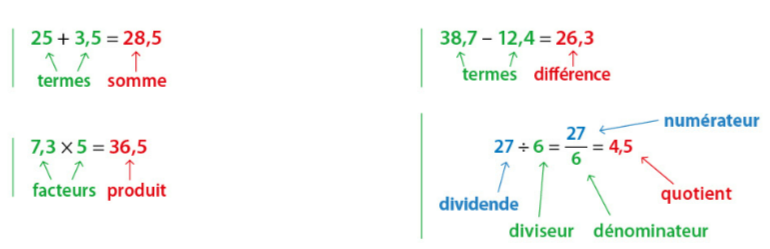
\includegraphics[width=1\linewidth]{../../assets/images/6e/seq_01/vocabualire_operations}
\end{center}
\end{examplebox}

\begin{definitionbox}
La nature d'une expression comportant plusieurs opérations est déterminée par l'opération effectuée en dernier.
\end{definitionbox}

\begin{examplebox}
Dans l'expression $2 + 3 \times 5$, c'est \trous{5cm} qu'on effectue en dernier, car la \trous{5cm} est prioritaire. Cette expression est donc une \trous{5cm}. C'est \trous{5cm} de $2$ et du \trous{5cm} de $3$ par $5$.
\end{examplebox}

\section{Exercices d'application}
\begin{exercisebox}
\textbf{Exercice 1 :} Calculer les expressions suivantes en détaillant les calculs.

\begin{enumerate}[label=\alph*)]
\item $A = 15 + 8 \times 3$
\item $B = 24 \div 6 + 5 \times 2$
\item $C = 10 - 3 \times 2 + 7$
\item $D = 18 \div (6 - 3) \times 4$
\end{enumerate}

\textbf{Exercice 2 :} Calculer les expressions suivantes.

\begin{enumerate}[label=\alph*)]
	\item $E = \frac{12 + 8}{5}$
	\item $F = \frac{30}{6 - 1}$
	\item $G = 5 \times (3 + 2 \times 4)$
	\item $H = [10 - (4 + 1)] \times 3$
\end{enumerate}

\textbf{Exercice 3 :} Identifier la nature de chaque expression (somme, différence, produit ou quotient).

\begin{enumerate}[label=\alph*)]
	\item $7 + 3 \times 2$
	\item $15 \div 3 + 4$
	\item $8 \times (5 - 2)$
	\item $\frac{20 + 4}{6}$
\end{enumerate}
\end{exercisebox}


 % Les nombres entiers
% Séquence 2 : Points et droites
\setseqtitle{Points et droites}
\chapter{Points et droites}
\label{chap:seq02}

% ======= Petits outils locaux (utilisables dans tout le chapitre) =======
% Pointillés pour les réponses (remplace \underline{\hspace{...}})
\newcommand{\trou}[1]{\makebox[#1]{\dotfill}}
% Styles TikZ (si déjà définis dans le préambule, ces lignes n'ont pas d'effet néfaste)
\tikzset{
	pt/.style   ={circle,fill=black,inner sep=1.2pt},
	lbl/.style  ={font=\footnotesize, inner sep=1pt},
	seg/.style  ={line width=0.9pt},
	dro/.style  ={line width=0.9pt},
	para/.style ={line width=0.9pt, dashed}
}

\begin{objectifsbox}
	\textbf{Vocabulaire et notations :} point, segment, demi-droite, droite, lectures [AB], (AB), [AB), AB.\\
	\textbf{Relations :} appartenance, alignement, droites sécantes/perpendiculaires/parallèles.\\
	\textbf{Méthodes :} tracer des parallèles et des perpendiculaires (règle + équerre).
\end{objectifsbox}

% =========================
\section*{1) Vocabulaire et notations}
\begin{itemize}
	\item Un point est un lieu dans le plan ; on le nomme par une \trou{5cm} majuscule.
	\item Une \trou{5cm} est une ligne définie par \trou{3cm} points distincts ; elle est \trou{3cm} (s'étend à l'infini).
	La droite passant par $A$ et $B$ se note : \trou{5cm}.
	\item Un \trou{3cm} est une portion de \trou{3cm} délimitée par deux \trou{3cm} appelés \trou{3cm}.
	On le note : \trou{3cm}.
	\item Une \trou{3cm} est une partie de \trou{2.2cm} qui commence en un \trou{3cm} donné et s'étend à l'infini.
	On la note par exemple : \trou{3cm}.
\end{itemize}

\textbf{Lecture :} $[AB]$ se lit << \trou{3cm} >> ; $(AB)$ se lit << \trou{3cm} >> ; $[AB)$ se lit << \trou{3cm} >> ;
$AB$ se lit << \trou{3cm} >> (ou << \trou{3cm} >>).

% --- Figure vocabulaire : droite, segment, demi-droite, longueur AB
\begin{figure}[h]
	\centering
	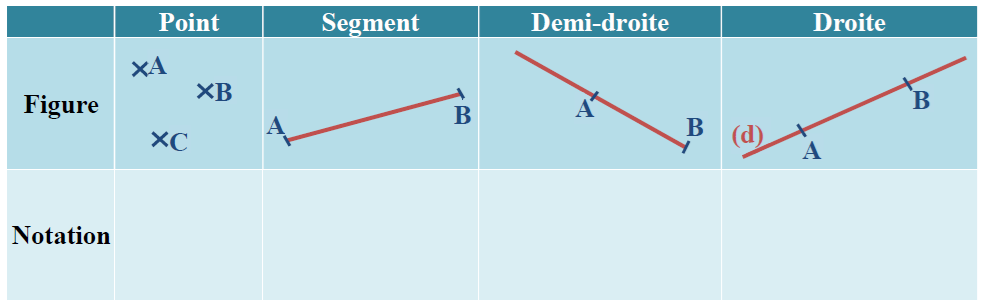
\includegraphics[width=1\linewidth]{../../../assets/images/6e/seq_02/points_segment_droites.png}
	\caption{Vocabulaire : $(AB)$ droite ; $[CD]$ segment ; $[EF)$ demi-droite ; $AB$ longueur.}
	\label{fig:vocab-points-droites}
\end{figure}

% =========================
\section*{2) Appartenance et alignement}
\begin{itemize}[label = \textbullet]
	\item $A$ \trou{1cm} $(d)$, $B$ \trou{1cm} $(d)$, $C$ \trou{1cm} $(d)$ ; $K$ \trou{1cm} $(d)$.
	\item Définition : Des points sont dits \textbf{alignés} s'ils \trou{6cm}.
\end{itemize}

% --- Figure appartenance et alignement
\begin{figure}[h]
	\centering
	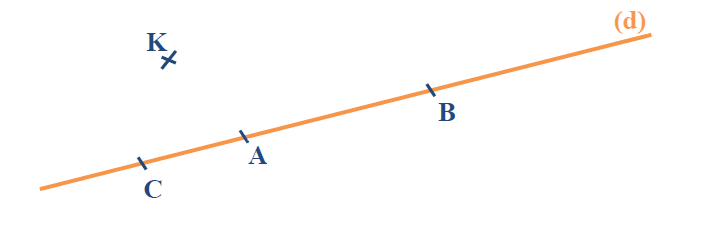
\includegraphics[width=1\linewidth]{../../../assets/images/6e/seq_02/pt_sur_dte.png}

	\label{fig:point-sur-droite}
\end{figure}

% =========================
\section*{3) Positions relatives des droites}
\begin{itemize}
	\item Deux droites sont \textbf{sécantes} si elles se coupent en \trou{1.2cm} point.
	\item Deux droites sont \textbf{perpendiculaires} si elles se coupent en formant un \trou{1.5cm} \trou{1.5cm}. On note : $(d)\perp(d')$.
	\item Deux droites sont \textbf{parallèles} si elles ne sont pas \trou{2.2cm}. On note : $(AB)//(EF)$.
\end{itemize}

\textbf{Lecture :} $(AB)//(EF)$ se lit << \trou{5cm} >> (ou << \trou{5cm} >>). \quad $(d)\perp(\Delta)$ se lit << \trou{5cm} >>.

% --- Figures sécantes / perpendiculaires / parallèles
\begin{figure}[h]
	\centering
	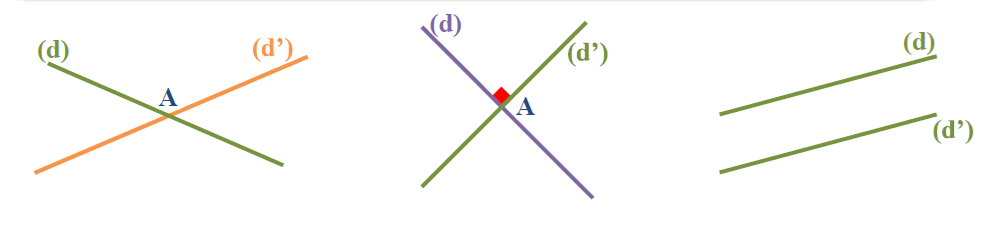
\includegraphics[width=1\linewidth]{../../../assets/images/6e/seq_02/position_relative.png}
	%\caption{Vocabulaire : $(AB)$ droite ; $[CD]$ segment ; $[EF)$ demi-droite ; $AB$ longueur.}
	\label{fig:Position relative de droites}
\end{figure}

% =========================
\section*{4) Tracer à la règle et à l'équerre}
\begin{itemize}
	\item Perpendiculaire à $(d)$ passant par $A$ : placer l'\trou{2.5cm} sur $(d)$, aligner le petit \trou{2.3cm}, faire un repère par $A$, tracer la droite \trou{2.3cm} à $(d)$.
	\item Parallèle à $(d)$ passant par $B$ : avec \trou{2.3cm} et équerre, faire glisser l'équerre en conservant le \trou{2.3cm} ; quand un côté passe par $B$, tracer la \trou{2.3cm} à $(d)$.
\end{itemize}

% --- Figures de construction : perpendiculaire en A, parallèle par B
\begin{figure}[h]
	\centering
	\begin{tikzpicture}[scale=1]
		% Perpendiculaire en A
		\begin{scope}[shift={(-4,0)}]
			\coordinate (A) at (-0.5,0.2);
			\coordinate (B) at (2,0);
			\draw[dro] (-2,0.15)--(2.2, -0.05); % (d)
			\node[lbl,below right] at (1.9,-0.05) {$(d)$};
			\node[pt] at (A) {}; \node[lbl,above] at (A) {$A$};
			% perpendiculaire
			\draw[dro] ($(A)!-1!(90:1)$) -- ($(A)!1!(90:1)$);
			\fill[gray!30] (A) -- ($(A)+(0.35,0)$) -- ($(A)+(0.35,0.35)$) -- ($(A)+(0,0.35)$) -- cycle;
			\node[lbl] at (-0.5,-0.7) {Perpendiculaire en $A$};
		\end{scope}
		
		% Parallèle par B
		\begin{scope}[shift={(3.5,0)}]
			\coordinate (P) at (-1.8,0.1);
			\coordinate (Q) at (1.8,-0.05);
			\draw[dro] (-2,0.1)--(2,-0.05); % (d)
			\node[lbl,below right] at (1.9,-0.08) {$(d)$};
			\coordinate (B) at (0.2,1.0);
			\node[pt] at (B) {}; \node[lbl,above] at (B) {$B$};
			% parallèle par B (même direction que (d))
			\draw[para] ($(B)+(-2,0.15)$)--($(B)+(2,0.0)$);
			\node[lbl] at (0.2,0.5) {Parallèle par $B$};
		\end{scope}
	\end{tikzpicture}
	\caption{Constructions : perpendiculaire en $A$ ; parallèle passant par $B$.}
	\label{fig:constructions}
\end{figure}

% =========================
\section*{5) Existence et unicité}
\begin{itemize}
	\item Par deux points distincts, il passe \trou{1.5cm} droite et une seule.
	\item Par un point donné $A$, il existe \trou{1.5cm} droite \trou{2cm} à $(d)$ ; elle est \trou{1.4cm}.
	\item Par un point donné $A$, il existe \trou{1.5cm} droite \trou{2cm} à $(d)$ ; elle est \trou{1.4cm}.
\end{itemize}

% =========================
\section*{6) Je m'entraîne}
\begin{itemize}
	\item Lecture : $[MN]$, $(RS)$, $[TU)$, $VU$.
	\item Notations : << La droite passant par $P$ et $Q$ >> ; << Le segment $KL$ >> ; << La demi-droite d'origine $H$ passant par $J$ >> ; << La longueur $AB$ >>.
	\item Complète : Si $A \in (BC)$ alors $A,B,C$ sont \trou{2cm}. Si $D \notin (EF)$ alors $D$ \trou{2cm} à la droite $(EF)$.
\end{itemize}
 % Points et droites
% Séquence 3 : Fractions décimales et nombres décimaux
\setseqtitle{Fractions décimales et nombres décimaux}
\chapter{Fractions décimales et nombres décimaux}

\begin{objectifsbox}
\textbf{Objectifs d'apprentissage.} À l'issue de la séquence, l'élève sera capable de :
\begin{itemize}
\item Reconnaître les fractions décimales
\item Convertir entre fractions décimales et nombres décimaux
\item Utiliser les nombres décimaux dans des calculs
\end{itemize}
\end{objectifsbox}

\section{Les fractions décimales}

\begin{definitionbox}
Une \textbf{fraction décimale} est une fraction dont le dénominateur est une puissance de 10.
\end{definitionbox}

\begin{examplebox}
\textbf{Exemples :} $\frac{3}{10}$, $\frac{25}{100}$, $\frac{7}{1000}$
\end{examplebox}

\section{Les nombres décimaux}

\begin{definitionbox}
Un \textbf{nombre décimal} est un nombre qui peut s'écrire avec une virgule.
\end{definitionbox}

\begin{proprietebox}
\textbf{Propriété :} $\frac{3}{10} = 0,3$ et $\frac{25}{100} = 0,25$
\end{proprietebox}

\begin{exercisebox}
\textbf{Exercice d'application :}
Convertir $\frac{7}{100}$ en nombre décimal.
\end{exercisebox}
 % Fractions décimales et nombres décimaux
% Séquence 4 : Distance, cercle et triangles
\setseqtitle{Distance, cercle et triangles}
\chapter{Distance, cercle et triangles}

\begin{objectifsbox}
	\textbf{Objectifs d'apprentissage de la séquence}
	\begin{itemize}
		\item Connaître et utiliser la définition de la distance entre deux points
		\item Connaître et utiliser la définition du milieu d'un segment
		\item Connaître les définitions d'un cercle, d'un disque, d'un rayon, d'un diamètre, d'une corde
		\item Comprendre la définition d'un cercle et celle d'un disque sous la forme d'ensembles de points
		\item Construire des triangles
		\item Résoudre des problèmes mettant en jeu des distances à un point
	\end{itemize}
\end{objectifsbox}

\section{Distance entre deux points}

\begin{definitionbox}
	\textbf{Distance entre deux points}
	
	La distance entre deux points A et B est \trous{5cm}.
	
	On la note \trous{3cm} et on peut également noter \trous{3cm}.
\end{definitionbox}

\textbf{Propriétés importantes :}
\begin{itemize}
	\item La distance entre deux points est toujours \trous{3cm}
	\item La distance d'un point A à un point B est \trous{5cm} que la distance du point B au point A
	\item On peut noter : \trous{4cm}
\end{itemize}

\textbf{Remarque :} Ne pas oublier l'unité de longueur !

\begin{examplebox}
	Soient 3 points O, P et M tels que OM = 3 cm, MP = 5 cm et OP = 8 cm.
	Montrer que le point M appartient au segment [OP].
	
	\trous{12cm}
	
	\trous{12cm}
	
	\trous{12cm}
\end{examplebox}

\section{Appartenance à un segment}

\begin{definitionbox}
	\textbf{Points et segments}
	
	Le segment [AB] est \trous{6cm}.
	
	Si le point C n'appartient pas au segment [AB], alors \trous{4cm}.
	
	Si le point D appartient au segment [AB], alors \trous{4cm}.
	
	Pour tout point M, \trous{4cm}.
\end{definitionbox}

Le symbole << $\geqslant$ >> se lit \trous{4cm}.

\textbf{Propriété :} Si AD + DB = AB, alors \trous{6cm}.

\section{Milieu d'un segment}

\begin{definitionbox}
	\textbf{Milieu d'un segment}
	
	Le milieu d'un segment est \trous{8cm}.
	
	<< Équidistant >> signifie << \trous{4cm} >>.
\end{definitionbox}

\begin{examplebox}
	% Schéma avec segment et milieu
	\begin{center}
		\begin{tikzpicture}[scale=1.2]
			% Segment RS avec milieu J
			\draw[thick] (0,0) -- (6,0);
			\fill (0,0) circle (0.1);
			\fill (6,0) circle (0.1);
			\fill (3,0) circle (0.1);
			
			\node[below] at (0,-0.3) {R};
			\node[below] at (6,-0.3) {S};
			\node[below] at (3,-0.3) {J};
			
			% Codage des segments égaux
			\draw (1.4,-0.1) -- (1.6,0.1);
			\draw (1.4,0.1) -- (1.6,-0.1);
			\draw (4.4,-0.1) -- (4.6,0.1);
			\draw (4.4,0.1) -- (4.6,-0.1);
		\end{tikzpicture}
	\end{center}
	
	J $\in$ [RS] et RJ = JS
	
	Donc \trous{6cm}
	
	Ne pas oublier le codage !
\end{examplebox}

\section{Le cercle}

\begin{definitionbox}
	\textbf{Définitions importantes}
	
	Le cercle de centre O et de rayon r est \trous{8cm}.
	
	Le disque de centre O et de rayon r est \trous{8cm}.
\end{definitionbox}

% Schéma d'un cercle avec vocabulaire
\begin{center}
	\begin{tikzpicture}[scale=1.2]
		% Cercle
		\draw[thick] (0,0) circle (2.5);
		
		% Centre
		\fill (0,0) circle (0.1);
		\node[below left] at (0,0) {O};
		
		% Rayon
		\draw[thick, red] (0,0) -- (1.77,1.77);
		\fill (1.77,1.77) circle (0.1);
		\node[above right] at (1.77,1.77) {A};
		
		% Diamètre
		\draw[thick, blue] (-2.5,0) -- (2.5,0);
		\fill (-2.5,0) circle (0.1);
		\fill (2.5,0) circle (0.1);
		\node[left] at (-2.5,0) {B};
		\node[right] at (2.5,0) {C};
		
		% Corde
		\draw[thick, green] (-1.5,2) -- (2,1.5);
		\fill (-1.5,2) circle (0.1);
		\fill (2,1.5) circle (0.1);
		\node[above] at (-1.5,2) {D};
		\node[above] at (2,1.5) {E};
	\end{tikzpicture}
\end{center}

\textbf{Vocabulaire :}
\begin{itemize}
	\item OA = \trous{3cm}
	\item [OA] est \trous{3cm}
	\item [BC] est \trous{3cm}
	\item [DE] est \trous{3cm}
	\item DE est \trous{3cm}
\end{itemize}

\section{Utilisation de la définition du cercle}

\begin{examplebox}
	\textbf{Exercice 1 :} Trace l'ensemble de tous les points situés à 5 cm du point O.
	
	\trous{10cm}
	
	\vspace{3cm}
	
	\textbf{Exercice 2 :} Trace et colorie l'ensemble de tous les points situés à plus de 2 cm et à moins de 4 cm du point P.
	
	\trous{10cm}
	
	\vspace{3cm}
\end{examplebox}

\section{Construction d'un triangle équilatéral}

\begin{definitionbox}
	\textbf{Triangle équilatéral}
	
	Un triangle équilatéral est un triangle qui a ses trois côtés de même mesure.
\end{definitionbox}

\textbf{Méthode de construction :}

Pour tracer un triangle équilatéral, on commence par tracer un côté puis, au compas, on trouve son troisième sommet.

\textbf{Points importants :}
\begin{itemize}
	\item On n'oublie pas de placer les noms des sommets
	\item On n'oublie pas le codage pour indiquer que les trois côtés ont la même mesure
	\item Les marques de construction doivent rester visibles
\end{itemize}

\begin{examplebox}
	\textbf{Exemple :} Finis la construction du triangle équilatéral LMN de côté 5 cm.
	
	% Schéma à compléter
	\begin{center}
		\begin{tikzpicture}[scale=1.2]
			% Segment LN déjà tracé
			\draw[thick] (0,0) -- (4,0);
			\fill (0,0) circle (0.1);
			\fill (4,0) circle (0.1);
			\node[below] at (0,-0.3) {L};
			\node[below] at (4,-0.3) {N};
			
			% Arcs de construction (en pointillés)
			\draw[dashed, red] (0,0) circle (4);
			\draw[dashed, blue] (4,0) circle (4);
		\end{tikzpicture}
	\end{center}
	
	\vspace{3cm}
\end{examplebox}

\section{Construction d'un triangle isocèle}

\begin{definitionbox}
	\textbf{Triangle isocèle}
	
	Un triangle isocèle est un triangle qui possède deux côtés de même mesure.
	
	Dire que le triangle ABC est isocèle en A revient à dire que A est son \trous{4cm} et donc que [BC] est sa \trous{3cm}.
	
	[AB] et [AC] sont donc de même mesure.
\end{definitionbox}

\textbf{Méthode de construction :}

Pour tracer un triangle isocèle, on commence par tracer sa base puis, au compas, on trouve son sommet principal.

\begin{examplebox}
	\textbf{Exemple :} Finis la construction du triangle ABC isocèle en A sachant que BC = 3 cm et AB = 5 cm.
	
	% Schéma à compléter
	\begin{center}
		\begin{tikzpicture}[scale=1.2]
			% Base BC déjà tracée
			\draw[thick] (0,0) -- (3,0);
			\fill (0,0) circle (0.1);
			\fill (3,0) circle (0.1);
			\node[below] at (0,-0.3) {B};
			\node[below] at (3,-0.3) {C};
			
			% Arc de construction depuis B
			\draw[dashed, red] (0,0) circle (5);
		\end{tikzpicture}
	\end{center}
	
	\vspace{3cm}
\end{examplebox}

\section{Construction d'un triangle quelconque}

\begin{definitionbox}
	\textbf{Triangle quelconque}
	
	Un triangle quelconque a ses 3 côtés de mesures différentes.
\end{definitionbox}

\textbf{Méthode de construction :}

Pour tracer un triangle quelconque, on commence par tracer son plus long côté. Le troisième sommet se trace avec un compas.

\begin{examplebox}
	\textbf{Exemple 1 :} Finis la construction du triangle ABC sachant que AC = 8 cm, AB = 6 cm et BC = 4 cm.
	
	% Schéma à compléter
	\begin{center}
		\begin{tikzpicture}[scale=1.2]
			% Le plus long côté AC déjà tracé
			\draw[thick] (0,0) -- (6,0);
			\fill (0,0) circle (0.1);
			\fill (6,0) circle (0.1);
			\node[below] at (0,-0.3) {A};
			\node[below] at (6,-0.3) {C};
			\node[above] at (3,0.2) {8 cm};
		\end{tikzpicture}
	\end{center}
	
	\vspace{3cm}
	
	\textbf{Exemple 2 :} Trace un triangle EFG sachant que EF = 10 cm, FG = 8 cm et EG = 5 cm.
	
	\vspace{4cm}
\end{examplebox}

\textbf{Remarques importantes :}
\begin{itemize}
	\item Les marques de construction doivent rester visibles
	\item Ne pas oublier de nommer les 3 sommets
\end{itemize}

\section{Construction d'un triangle rectangle}

\begin{definitionbox}
	\textbf{Triangle rectangle}
	
	Un triangle rectangle est un triangle qui possède un angle droit.
\end{definitionbox}

\textbf{Méthode de construction :}

Pour tracer un triangle rectangle, on commence par tracer les 2 côtés de l'angle droit avec une règle et une équerre puis on reporte les longueurs connues.

\textbf{Points importants :}
\begin{itemize}
	\item On n'oublie pas de placer les noms des sommets
	\item On n'oublie pas le codage pour indiquer l'angle droit
\end{itemize}

\begin{examplebox}
	\textbf{Exemple 1 :} Finis la construction du triangle ABC rectangle en C sachant que AC = 5 cm et BC = 4 cm.
	
	% Schéma à compléter
	\begin{center}
		\begin{tikzpicture}[scale=1.2]
			% Angle droit en C
			\draw[thick] (0,0) -- (4,0);
			\draw[thick] (0,0) -- (0,3);
			\fill (0,0) circle (0.1);
			\node[below left] at (0,0) {C};
			
			% Codage angle droit
			\draw (0.3,0) -- (0.3,0.3) -- (0,0.3);
		\end{tikzpicture}
	\end{center}
	
	\vspace{3cm}
	
	\textbf{Exemple 2 : les 2 côtés de l'angle droit sont connus}
	
	Trace un triangle EFG rectangle en F sachant que EF = 6 cm et FG = 2 cm.
	
	\vspace{3cm}
	
	\textbf{Exemple 3 : un seul côté de l'angle droit est connu}
	
	Trace un triangle MNO rectangle en O sachant que ON = 3 cm et MN = 5 cm.
	
	\vspace{3cm}
\end{examplebox}

\textbf{Exercices d'application :}

\begin{exercisebox}
	1. Construire un triangle équilatéral XYZ de côté 3,5 cm.
	
	\vspace{4cm}
	
	2. Construire un triangle IJK isocèle en J avec IJ = 7 cm et IK = 4 cm.
	
	\vspace{4cm}
	
	3. Les points A, B et C sont-ils alignés si AB = 5 cm, BC = 3 cm et AC = 8 cm ? Justifier.
	
	\trous{8cm}
	
	\trous{8cm}
	
	4. Soit M le milieu du segment [EF]. Si EM = 3,5 cm, quelle est la longueur EF ?
	
	\trous{8cm}
\end{exercisebox} % Distance, cercle et triangles
% Séquence 5 : Notion de proportionnalité
\setseqtitle{Notion de proportionnalité}
\chapter{Notion de proportionnalité}
\label{chap:seq05}

\begin{definitionbox}
\textbf{Objectifs d'apprentissage.} À l'issue de la séquence, l'élève sera capable de :
\begin{itemize}
  \item ...
\end{itemize}
\end{definitionbox}

\section*{Pré-requis}
\begin{itemize}
  \item ...
\end{itemize}

\section{Découverte}
\begin{examplebox}
Problème d'introduction ou situation de découverte.
\end{examplebox}

\section{Leçon}
\begin{itemize}
  \item Rappels et définitions.
  \item Méthodes et exemples guidés.
\end{itemize}

\section{Exercices d'entraînement}
\begin{exercisebox}
Exercice 1.
\end{exercisebox}

\begin{exercisebox}
Exercice 2.
\end{exercisebox}

\section{Évaluation rapide (5 à 10 min)}
\begin{exercisebox}
Mini-quiz.
\end{exercisebox}
 % Notion de proportionnalité
% Séquence 6 : Notion de probabilités
\chapter{Notion de probabilités}
\label{chap:seq06}

\begin{definitionbox}
\textbf{Objectifs d'apprentissage.} À l'issue de la séquence, l'élève sera capable de :
\begin{itemize}
  \item ...
\end{itemize}
\end{definitionbox}

\section*{Pré-requis}
\begin{itemize}
  \item ...
\end{itemize}

\section{Découverte}
\begin{examplebox}
Problème d'introduction ou situation de découverte.
\end{examplebox}

\section{Leçon}
\begin{itemize}
  \item Rappels et définitions.
  \item Méthodes et exemples guidés.
\end{itemize}

\section{Exercices d'entraînement}
\begin{exercisebox}
Exercice 1.
\end{exercisebox}

\begin{exercisebox}
Exercice 2.
\end{exercisebox}

\section{Évaluation rapide (5 à 10 min)}
\begin{exercisebox}
Mini-quiz.
\end{exercisebox}
 % Notion de probabilités
% Séquence 7 : Angles et rapporteur
\chapter{Angles et rapporteur}
\label{chap:seq07}

\begin{definitionbox}
\textbf{Objectifs d'apprentissage.} À l'issue de la séquence, l'élève sera capable de :
\begin{itemize}
  \item ...
\end{itemize}
\end{definitionbox}

\section*{Pré-requis}
\begin{itemize}
  \item ...
\end{itemize}

\section{Découverte}
\begin{examplebox}
Problème d'introduction ou situation de découverte.
\end{examplebox}

\section{Leçon}
\begin{itemize}
  \item Rappels et définitions.
  \item Méthodes et exemples guidés.
\end{itemize}

\section{Exercices d'entraînement}
\begin{exercisebox}
Exercice 1.
\end{exercisebox}

\begin{exercisebox}
Exercice 2.
\end{exercisebox}

\section{Évaluation rapide (5 à 10 min)}
\begin{exercisebox}
Mini-quiz.
\end{exercisebox}
 % Angles et rapporteur
\setseqtitle{Opérations avec les nombres décimaux}
\chapter{Opérations avec les nombres décimaux}
\label{chap:seq08}

\begin{objectifsbox}
\textbf{Objectifs d'apprentissage.} À l'issue de la séquence, l'élève sera capable de :
\begin{itemize}
  \item Additionner et soustraire des nombres décimaux
  \item Multiplier des nombres décimaux
  \item Poser correctement les opérations avec des nombres décimaux
  \item Calculer des ordres de grandeur
\end{itemize}
\end{objectifsbox}

\section*{Pré-requis}
\begin{itemize}
  \item Connaissance des nombres entiers et de leurs opérations
  \item Maîtrise de la numération décimale
  \item Compréhension de la valeur des chiffres selon leur position
\end{itemize}

\section{Addition et soustraction avec des nombres décimaux}

\begin{definitionbox}
	\textbf{Addition et soustraction}
	
	On calcule une \textbf{\trous{3cm}} lorsqu'on ajoute deux nombres, et une \textbf{\trous{3cm}} lorsqu'on en soustrait deux.
	
	Le résultat d'une addition est une \textbf{\trous{2.5cm}}, celui d'une soustraction une \textbf{\trous{2.5cm}}.
	
	Les nombres calculés ensemble s'appellent les \textbf{\trous{2.5cm}}.
\end{definitionbox}

\begin{examplebox}
	\begin{center}
		\begin{tabular}{p{0.45\textwidth}p{0.45\textwidth}}
			\textbf{21,5 + 12,3 = 33,8} (\trous{2.5cm}) & \textbf{21,5 - 12,3 = 9,2} (\trous{2.5cm}) \\
			On dit que << 33,8 est la somme de 21,5 et 12,3 >> & On dit que << 9,2 est la différence de 21,5 par 12,3 >> \\
		\end{tabular}
	\end{center}
	
	Dans les deux cas, les deux nombres \textbf{21,5} et \textbf{12,3} sont les \textbf{termes} du calcul.
\end{examplebox}

\begin{proprietebox}
On peut échanger les termes d'une addition sans modifier son résultat. On dit que l'addition est \textbf{\trous{3cm}}.
\end{proprietebox}

\textbf{ATTENTION :} Ce n'est pas vrai pour une soustraction !

% Exemple 1 : opération en ligne dans une boxe
\begin{examplebox}
	\begin{center}
		\begin{tabular}{p{0.45\textwidth} p{0.45\textwidth}}
			\textbf{Exemple 1 (opération en ligne)} : \\
			$8,5 + 7,2 + 2,1 + 3,4$ & $8,5 - 3,2$ \\
			$= \underline{\trous{1cm} + \trous{1cm}} + \underline{\trous{1cm} + \trous{1cm}}$ & $= 5,3$ \\
			$= 10,6 + 10,6$ & (attention : on ne sait pas encore calculer $3,2 - 8,5$) \\
			$= 21,2$ & \\
		\end{tabular}
	\end{center}
\end{examplebox}

\vspace{0.5cm}

% Exemple 2 : opération posée dans une boxe
\begin{examplebox}
	\begin{center}
		\begin{tabular}{p{0.45\textwidth} p{0.45\textwidth}}
			\textbf{Exemple 2 (opération posée)} : \underline{\textbf{28,4 + 84,39}} 
			& 
			\underline{\textbf{20,18 - 19,45}} \\
			
			\begin{tabular}{r}
				84,39 \\
				+ 28,40 \\
				\hline
				\trous{1.5cm}
			\end{tabular} &
			\begin{tabular}{r}
				20,18 \\
				- 19,45 \\
				\hline
				\trous{1.5cm}
			\end{tabular} \\
			
		\end{tabular}
	\end{center}
\end{examplebox}


\textbf{Remarques :}
\begin{itemize}
	\item Les mots << \textbf{addition} >> et << \textbf{soustraction} >> désignent des opérations, tandis que les mots << \textbf{somme} >> et << \textbf{différence} >> désignent des nombres (des résultats).
	\item Pour poser une addition ou une soustraction de nombres décimaux, il faut impérativement aligner les nombres par la droite et aligner les virgules.
	\item On peut ajouter des zéros à droite d'un nombre décimal sans changer sa valeur (exemple : 28,4 = 28,40).
\end{itemize}

\section{Multiplication avec des nombres décimaux}

\begin{definitionbox}
	\textbf{Multiplication}
	
	Dans une \textbf{multiplication}, on multiplie des \trous{2.5cm}, et le résultat est un \trous{2cm}.
\end{definitionbox}

\begin{examplebox}
	On dit que 60,5 est le \trous{2.5cm} de 12,1 par 5
\end{examplebox}

\begin{proprietebox}
On peut échanger l'ordre des facteurs sans changer le résultat. On dit que la multiplication est \trous{3cm}.
\end{proprietebox}

\textbf{Méthode :} Poser une multiplication avec des nombres décimaux.

\textbf{Exemple :} $25,1 \times 7,53$

\begin{center}
	\begin{tabular}{r}
		25,1 \\
		$\times$ 7,53 \\
		\hline
		\trous{2cm} \\
		\trous{2cm} \\
		\trous{2cm} \\
		\hline
		\trous{2cm}
	\end{tabular}
\end{center}

\textbf{Règle pour placer la virgule :} Le nombre de chiffres après la virgule dans le résultat est égal à la somme du nombre de chiffres après la virgule dans chaque facteur.

\section{Ordre de grandeur}

\begin{definitionbox}
	\textbf{Ordre de grandeur}
	
	Un \textbf{ordre de grandeur} d'un nombre est un nombre proche de celui-ci et facile à utiliser en calcul mental.
	
	\textbf{Remarque :} Un ordre de grandeur n'est pas unique : on peut donner des ordres de grandeur différents selon la précision voulue.
\end{definitionbox}

\begin{examplebox}
	La population française était de 67 063 703 habitants en 2020. Un ordre de grandeur de cette population est \trous{3cm} (on pourrait aussi choisir 100 millions ou 67 millions).
\end{examplebox}

\begin{examplebox}
Pour calculer $24,7 \times 3,8$, on peut d'abord estimer :

• 24,7 $\approx$ 25 (ordre de grandeur)

• 3,8 $\approx$ 4 (ordre de grandeur)

• Donc $24,7 \times 3,8 \approx 25 \times 4 = 100$

Le résultat exact sera proche de 100.
\end{examplebox}

\section{Exercices d'entraînement}

\begin{exercisebox}
\textbf{Exercices d'application :} Pose et calcule les opérations suivantes :
\begin{enumerate}
	\item 45,7 + 23,8
	\item 67,2 - 34,5
	\item $12,3 \times 4,6$
\end{enumerate}
\end{exercisebox}

\begin{exercisebox}
\textbf{Exercices d'application :} Donne un ordre de grandeur de chaque calcul, puis calcule le résultat exact :
\begin{enumerate}
	\item 23,4 + 45,7
	\item 89,2 - 12,8
	\item $15,6 \times 3,2$
\end{enumerate}
\end{exercisebox}

\section{Évaluation rapide (5 à 10 min)}

\begin{exercisebox}
\textbf{Évaluation rapide :}
\begin{enumerate}
	\item Quel est le résultat de 12,5 + 8,7 ?
	\item Calcule 45,2 - 23,8
	\item Donne un ordre de grandeur de $34,7 \times 2,1$
\end{enumerate}
\end{exercisebox}
 % Opérations avec les nombres décimaux
\chapter{La médiatrice d’un segment}
\label{chap:seq09}

\begin{definitionbox}
\textbf{Objectifs d'apprentissage.} À l'issue de la séquence, l'élève sera capable de :
\begin{itemize}
  \item ...
\end{itemize}
\end{definitionbox}

\section*{Pré-requis}
\begin{itemize}
  \item ...
\end{itemize}

\section{Découverte}
\begin{examplebox}
Problème d'introduction ou situation de découverte.
\end{examplebox}

\section{Leçon}
\begin{itemize}
  \item Rappels et définitions.
  \item Méthodes et exemples guidés.
\end{itemize}

\section{Exercices d'entraînement}
\begin{exercisebox}
Exercice 1.
\end{exercisebox}

\begin{exercisebox}
Exercice 2.
\end{exercisebox}

\section{Évaluation rapide (5 à 10 min)}
\begin{exercisebox}
Mini-quiz.
\end{exercisebox}
 % La médiatrice d'un segment
\chapter{La division}
\label{chap:seq10}

\begin{definitionbox}
\textbf{Objectifs d'apprentissage.} À l'issue de la séquence, l'élève sera capable de :
\begin{itemize}
  \item ...
\end{itemize}
\end{definitionbox}

\section*{Pré-requis}
\begin{itemize}
  \item ...
\end{itemize}

\section{Découverte}
\begin{examplebox}
Problème d'introduction ou situation de découverte.
\end{examplebox}

\section{Leçon}
\begin{itemize}
  \item Rappels et définitions.
  \item Méthodes et exemples guidés.
\end{itemize}

\section{Exercices d'entraînement}
\begin{exercisebox}
Exercice 1.
\end{exercisebox}

\begin{exercisebox}
Exercice 2.
\end{exercisebox}

\section{Évaluation rapide (5 à 10 min)}
\begin{exercisebox}
Mini-quiz.
\end{exercisebox}
 % La division
\chapter{Symétrie axiale}
\label{chap:seq11}

\begin{definitionbox}
\textbf{Objectifs d'apprentissage.} À l'issue de la séquence, l'élève sera capable de :
\begin{itemize}
  \item ...
\end{itemize}
\end{definitionbox}

\section*{Pré-requis}
\begin{itemize}
  \item ...
\end{itemize}

\section{Découverte}
\begin{examplebox}
Problème d'introduction ou situation de découverte.
\end{examplebox}

\section{Leçon}
\begin{itemize}
  \item Rappels et définitions.
  \item Méthodes et exemples guidés.
\end{itemize}

\section{Exercices d'entraînement}
\begin{exercisebox}
Exercice 1.
\end{exercisebox}

\begin{exercisebox}
Exercice 2.
\end{exercisebox}

\section{Évaluation rapide (5 à 10 min)}
\begin{exercisebox}
Mini-quiz.
\end{exercisebox}
 % Symétrie axiale
\chapter{Fraction partage et comparaison de fractions}
\label{chap:seq12}

\begin{definitionbox}
\textbf{Objectifs d'apprentissage.} À l'issue de la séquence, l'élève sera capable de :
\begin{itemize}
  \item ...
\end{itemize}
\end{definitionbox}

\section*{Pré-requis}
\begin{itemize}
  \item ...
\end{itemize}

\section{Découverte}
\begin{examplebox}
Problème d'introduction ou situation de découverte.
\end{examplebox}

\section{Leçon}
\begin{itemize}
  \item Rappels et définitions.
  \item Méthodes et exemples guidés.
\end{itemize}

\section{Exercices d'entraînement}
\begin{exercisebox}
Exercice 1.
\end{exercisebox}

\begin{exercisebox}
Exercice 2.
\end{exercisebox}

\section{Évaluation rapide (5 à 10 min)}
\begin{exercisebox}
Mini-quiz.
\end{exercisebox}
 % Fraction partage et comparaison de fractions
\chapter{Unités de longueur, de masse et de contenance}
\label{chap:seq13}

\begin{definitionbox}
\textbf{Objectifs d'apprentissage.} À l'issue de la séquence, l'élève sera capable de :
\begin{itemize}
  \item ...
\end{itemize}
\end{definitionbox}

\section*{Pré-requis}
\begin{itemize}
  \item ...
\end{itemize}

\section{Découverte}
\begin{examplebox}
Problème d'introduction ou situation de découverte.
\end{examplebox}

\section{Leçon}
\begin{itemize}
  \item Rappels et définitions.
  \item Méthodes et exemples guidés.
\end{itemize}

\section{Exercices d'entraînement}
\begin{exercisebox}
Exercice 1.
\end{exercisebox}

\begin{exercisebox}
Exercice 2.
\end{exercisebox}

\section{Évaluation rapide (5 à 10 min)}
\begin{exercisebox}
Mini-quiz.
\end{exercisebox}
 % Unités de longueur, de masse et de contenance
\chapter{Calculer avec les angles}
\label{chap:seq14}

\begin{definitionbox}
\textbf{Objectifs d'apprentissage.} À l'issue de la séquence, l'élève sera capable de :
\begin{itemize}
  \item ...
\end{itemize}
\end{definitionbox}

\section*{Pré-requis}
\begin{itemize}
  \item ...
\end{itemize}

\section{Découverte}
\begin{examplebox}
Problème d'introduction ou situation de découverte.
\end{examplebox}

\section{Leçon}
\begin{itemize}
  \item Rappels et définitions.
  \item Méthodes et exemples guidés.
\end{itemize}

\section{Exercices d'entraînement}
\begin{exercisebox}
Exercice 1.
\end{exercisebox}

\begin{exercisebox}
Exercice 2.
\end{exercisebox}

\section{Évaluation rapide (5 à 10 min)}
\begin{exercisebox}
Mini-quiz.
\end{exercisebox}
 % Calculer avec les angles
\chapter{Nombres en écriture fractionnaire}
\label{chap:seq15}

\begin{definitionbox}
\textbf{Objectifs d'apprentissage.} À l'issue de la séquence, l'élève sera capable de :
\begin{itemize}
  \item ...
\end{itemize}
\end{definitionbox}

\section*{Pré-requis}
\begin{itemize}
  \item ...
\end{itemize}

\section{Découverte}
\begin{examplebox}
Problème d'introduction ou situation de découverte.
\end{examplebox}

\section{Leçon}
\begin{itemize}
  \item Rappels et définitions.
  \item Méthodes et exemples guidés.
\end{itemize}

\section{Exercices d'entraînement}
\begin{exercisebox}
Exercice 1.
\end{exercisebox}

\begin{exercisebox}
Exercice 2.
\end{exercisebox}

\section{Évaluation rapide (5 à 10 min)}
\begin{exercisebox}
Mini-quiz.
\end{exercisebox}
 % Nombres en écriture fractionnaire
\chapter{Proportionnalité et pourcentages}
\label{chap:seq16}

\begin{definitionbox}
\textbf{Objectifs d'apprentissage.} À l'issue de la séquence, l'élève sera capable de :
\begin{itemize}
  \item ...
\end{itemize}
\end{definitionbox}

\section*{Pré-requis}
\begin{itemize}
  \item ...
\end{itemize}

\section{Découverte}
\begin{examplebox}
Problème d'introduction ou situation de découverte.
\end{examplebox}

\section{Leçon}
\begin{itemize}
  \item Rappels et définitions.
  \item Méthodes et exemples guidés.
\end{itemize}

\section{Exercices d'entraînement}
\begin{exercisebox}
Exercice 1.
\end{exercisebox}

\begin{exercisebox}
Exercice 2.
\end{exercisebox}

\section{Évaluation rapide (5 à 10 min)}
\begin{exercisebox}
Mini-quiz.
\end{exercisebox}
 % Proportionnalité et pourcentages
\chapter{Déterminer des probabilités et des issues}
\label{chap:seq17}

\begin{definitionbox}
\textbf{Objectifs d'apprentissage.} À l'issue de la séquence, l'élève sera capable de :
\begin{itemize}
  \item ...
\end{itemize}
\end{definitionbox}

\section*{Pré-requis}
\begin{itemize}
  \item ...
\end{itemize}

\section{Découverte}
\begin{examplebox}
Problème d'introduction ou situation de découverte.
\end{examplebox}

\section{Leçon}
\begin{itemize}
  \item Rappels et définitions.
  \item Méthodes et exemples guidés.
\end{itemize}

\section{Exercices d'entraînement}
\begin{exercisebox}
Exercice 1.
\end{exercisebox}

\begin{exercisebox}
Exercice 2.
\end{exercisebox}

\section{Évaluation rapide (5 à 10 min)}
\begin{exercisebox}
Mini-quiz.
\end{exercisebox}
 % Déterminer des probabilités et des issues
\chapter{Aires et périmètres}
\label{chap:seq18}

\begin{definitionbox}
\textbf{Objectifs d'apprentissage.} À l'issue de la séquence, l'élève sera capable de :
\begin{itemize}
  \item ...
\end{itemize}
\end{definitionbox}

\section*{Pré-requis}
\begin{itemize}
  \item ...
\end{itemize}

\section{Découverte}
\begin{examplebox}
Problème d'introduction ou situation de découverte.
\end{examplebox}

\section{Leçon}
\begin{itemize}
  \item Rappels et définitions.
  \item Méthodes et exemples guidés.
\end{itemize}

\section{Exercices d'entraînement}
\begin{exercisebox}
Exercice 1.
\end{exercisebox}

\begin{exercisebox}
Exercice 2.
\end{exercisebox}

\section{Évaluation rapide (5 à 10 min)}
\begin{exercisebox}
Mini-quiz.
\end{exercisebox}
 % Aires et périmètres
\chapter{Heures et durées}
\label{chap:seq19}

\begin{definitionbox}
\textbf{Objectifs d'apprentissage.} À l'issue de la séquence, l'élève sera capable de :
\begin{itemize}
  \item ...
\end{itemize}
\end{definitionbox}

\section*{Pré-requis}
\begin{itemize}
  \item ...
\end{itemize}

\section{Découverte}
\begin{examplebox}
Problème d'introduction ou situation de découverte.
\end{examplebox}

\section{Leçon}
\begin{itemize}
  \item Rappels et définitions.
  \item Méthodes et exemples guidés.
\end{itemize}

\section{Exercices d'entraînement}
\begin{exercisebox}
Exercice 1.
\end{exercisebox}

\begin{exercisebox}
Exercice 2.
\end{exercisebox}

\section{Évaluation rapide (5 à 10 min)}
\begin{exercisebox}
Mini-quiz.
\end{exercisebox}
 % Heures et durées
\chapter{Solides et volumes}
\label{chap:seq20}

\begin{definitionbox}
\textbf{Objectifs d'apprentissage.} À l'issue de la séquence, l'élève sera capable de :
\begin{itemize}
  \item ...
\end{itemize}
\end{definitionbox}

\section*{Pré-requis}
\begin{itemize}
  \item ...
\end{itemize}

\section{Découverte}
\begin{examplebox}
Problème d'introduction ou situation de découverte.
\end{examplebox}

\section{Leçon}
\begin{itemize}
  \item Rappels et définitions.
  \item Méthodes et exemples guidés.
\end{itemize}

\section{Exercices d'entraînement}
\begin{exercisebox}
Exercice 1.
\end{exercisebox}

\begin{exercisebox}
Exercice 2.
\end{exercisebox}

\section{Évaluation rapide (5 à 10 min)}
\begin{exercisebox}
Mini-quiz.
\end{exercisebox}
 % Solides et volumes


%\cleardoublepage
%\part{Géométrie}







%\cleardoublepage
%\part{Grandeurs et mesures}


%\cleardoublepage
%\part{Organisation et gestion de données \& Probabilités}




%\cleardoublepage

\appendix
\chapter{Progression annuelle (récapitulatif)}
Cette progression correspond à la répartition établie pour l'année 2025–2026.

\begin{center}
\begin{tabular}{|l|l|}
\hline
\textbf{Période} & \textbf{Séquences}\\ \hline
Période 1 (6 semaines) & S01 -- Les nombres entiers, S02 -- Points et droites, S03 -- Fractions décimales et nombres décimaux\\ \hline
Période 2 (7 semaines) & S04 -- Distance, cercle et triangles, S05 -- Notion de proportionnalité, S06 -- Notion de probabilités, S07 -- Angles et rapporteur\\ \hline
Période 3 (6 semaines) & S08 -- Opérations avec les nombres décimaux, S09 -- La médiatrice d'un segment, S10 -- La division, S11 -- Symétrie axiale\\ \hline
Période 4 (7 semaines) & S12 -- Fraction partage et comparaison de fractions, S13 -- Unités de longueur, de masse et de contenance, S14 -- Calculer avec les angles, S15 -- Nombres en écriture fractionnaire\\ \hline
Période 5 (6 semaines) & S16 -- Proportionnalité et pourcentages, S17 -- Déterminer des probabilités et des issues, S18 -- Aires et périmètres, S19 -- Heures et durées, S20 -- Solides et volumes\\ \hline
\end{tabular}
\end{center}

\end{document}
